\documentclass[aspectratio=169, 11pt]{beamer}

% ── Theme & Colors ──────────────────────────────────────────
\usetheme{Madrid}
\usecolortheme{default}

\definecolor{darkcharcoal}{HTML}{2C3E50}
\definecolor{accentblue}{HTML}{2980B9}
\definecolor{donegreen}{HTML}{27AE60}
\definecolor{pendinggray}{HTML}{BDC3C7}
\definecolor{lightbg}{HTML}{F8F9FA}
\definecolor{darktext}{HTML}{1A1A2E}

\setbeamercolor{structure}{fg=darkcharcoal}
\setbeamercolor{palette primary}{bg=darkcharcoal, fg=white}
\setbeamercolor{palette secondary}{bg=accentblue, fg=white}
\setbeamercolor{frametitle}{bg=darkcharcoal, fg=white}
\setbeamercolor{title}{fg=darkcharcoal}
\setbeamercolor{subtitle}{fg=accentblue}
\setbeamercolor{block title}{bg=darkcharcoal, fg=white}
\setbeamercolor{block body}{bg=lightbg, fg=darktext}
\setbeamercolor{item}{fg=accentblue}

\setbeamertemplate{navigation symbols}{}
\setbeamerfont{frametitle}{size=\large, series=\bfseries}
\setbeamerfont{title}{size=\Large, series=\bfseries}

% ── Packages ────────────────────────────────────────────────
\usepackage{tikz}
\usetikzlibrary{shapes.geometric, arrows.meta, positioning, fit, calc}
\usepackage{amsmath, amssymb}
\usepackage{booktabs}
\usepackage{graphicx}
\usepackage{hyperref}
\usepackage{xcolor}
\usepackage{array}

% ── TikZ Styles ─────────────────────────────────────────────
\tikzstyle{block} = [rectangle, rounded corners, minimum width=2.2cm, minimum height=0.8cm, text centered, draw=darkcharcoal, fill=lightbg, font=\small]
\tikzstyle{done} = [block, draw=donegreen, fill=donegreen!10, text=donegreen!80!black]
\tikzstyle{pending} = [block, draw=pendinggray, fill=pendinggray!15, text=pendinggray!60!black]
\tikzstyle{arrow} = [-{Stealth[length=2.5mm]}, thick, color=darkcharcoal!70]

% ── Meta ────────────────────────────────────────────────────
\title{Optimising Fed-Batch Bioprocesses using pyFOOMB}
\subtitle{UG Project Progress Report}
\author{Yashashwi Singhania }
% \institute{Department of Biochemical Engineering\\Indian Institute of Technology (BHU), Varanasi}
\date{April 2026}

% ═══════════════════════════════════════════════════════════
\begin{document}

% ── Slide 1: Title ──────────────────────────────────────────
\begin{frame}[plain]
  \vfill
  \begin{center}
    
\includegraphics[height=2.2cm]{iit_bhu_logo.png}\\[0.5cm]
    {\Large\bfseries\color{darkcharcoal} Indian Institute of Technology (BHU), Varanasi}\\[0.6cm]
    {\LARGE\bfseries\color{darkcharcoal} Optimising Fed-Batch Bioprocesses}\\[0.15cm]
    {\LARGE\bfseries\color{darkcharcoal} using pyFOOMB}\\[0.4cm]
    {\large\color{accentblue} UG Project Progress Report}\\[0.8cm]
    \begin{tabular}{rl}
      \textbf{Student:} & Yashashwi Singhania (23014019) \\
      \textbf{Guide:} & Dr.\ Sharon Mano Pappu J. \\
      \textbf{Department:} & Biochemical Engineering \\
      \textbf{Lab:} & BPDD (\_\_\_\_\_\_\_\_) \\
    \end{tabular}\\[0.5cm]
    {\small April 2026}
  \end{center}
  \vfill
\end{frame}

% ── Slide 2: Project Overview ───────────────────────────────
\begin{frame}{Project Overview}
  \begin{block}{Objective}
    Optimise the \textbf{fed-batch feeding strategy} for recombinant protein production
    by exploiting the relationship between specific growth rate ($\mu$) and
    specific product formation rate ($q_p$).
  \end{block}

  \vspace{0.3cm}
  \begin{columns}[T]
    \begin{column}{0.48\textwidth}
      \textbf{This Semester — Completed:}
      \begin{itemize}
        \item[\textcolor{donegreen}{\checkmark}] Studied the pyFOOMB framework
        \item[\textcolor{donegreen}{\checkmark}] Built a full web-based GUI
        \item[\textcolor{donegreen}{\checkmark}] Surveyed $\mu$--$q_p$ models from literature
        \item[\textcolor{donegreen}{\checkmark}] Simulated batch X, S, P profiles
      \end{itemize}
    \end{column}
    \begin{column}{0.48\textwidth}
      \textbf{Next Steps:}
      \begin{itemize}
        \item[\textcolor{pendinggray}{$\circ$}] Implement fed-batch models in pyFOOMB
        \item[\textcolor{pendinggray}{$\circ$}] Parameter estimation \& feed optimisation
        \item[\textcolor{pendinggray}{$\circ$}] Validate with experimental data
        \item[\textcolor{pendinggray}{$\circ$}] Deploy GUI
        \item[\textcolor{pendinggray}{$\circ$}] Scale-up analysis
      \end{itemize}
    \end{column}
  \end{columns}
\end{frame}

% ── Slide 3: What is pyFOOMB? ──────────────────────────────
\begin{frame}{What is pyFOOMB?}
  \textbf{Py}thon \textbf{F}ramework for \textbf{O}bject-\textbf{O}riented \textbf{M}odelling of \textbf{B}ioprocesses

  \vspace{0.2cm}
  {\small Hemmerich et al.\ (2021), \textit{Eng.\ Life Sci.}\ 21(3-4):242--257}

  \vspace{0.3cm}
  \begin{columns}[T]
    \begin{column}{0.55\textwidth}
      \textbf{Core Capabilities:}
      \begin{itemize}
        \item ODE-based bioprocess modelling
        \item User-defined kinetics in \texttt{rhs()} method
        \item Event handling for fed-batch (feed start/stop, bolus)
        \item Forward simulation via CVode (SUNDIALS)
        \item Parameter estimation: local (scipy) \& global (pygmo)
        \item Sensitivity analysis, FIM, OED
      \end{itemize}
    \end{column}
    \begin{column}{0.42\textwidth}
      \textbf{Key Difference:}
      \begin{block}{}
        pyFOOMB does \textbf{not} hardcode kinetic models.
        Users implement \textit{any} $\mu$--$q_p$ relationship
        in their model's \texttt{rhs()} method. The framework handles
        simulation, events, and estimation.
      \end{block}
    \end{column}
  \end{columns}
\end{frame}

% ── Slide 4: pyFOOMB Architecture ──────────────────────────
\begin{frame}{pyFOOMB Architecture}
  \begin{center}
  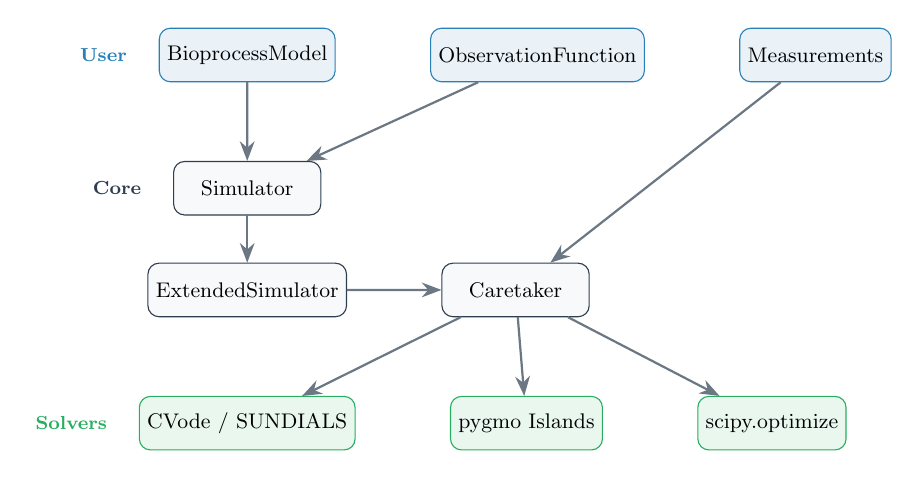
\begin{tikzpicture}[node distance=0.6cm and 1.2cm, scale=0.85, every node/.style={scale=0.85}]
    % User layer
    \node[block, fill=accentblue!10, draw=accentblue] (model) {BioprocessModel};
    \node[block, fill=accentblue!10, draw=accentblue, right=of model] (obs) {ObservationFunction};
    \node[block, fill=accentblue!10, draw=accentblue, right=of obs] (data) {Measurements};

    % Core layer
    \node[block, below=1cm of model] (sim) {Simulator};
    \node[block, below=of sim] (esim) {ExtendedSimulator};
    \node[block, right=of esim] (care) {Caretaker};

    % Engine layer
    \node[block, fill=donegreen!10, draw=donegreen, below=1cm of esim] (cvode) {CVode / SUNDIALS};
    \node[block, fill=donegreen!10, draw=donegreen, right=of cvode] (pygmo) {pygmo Islands};
    \node[block, fill=donegreen!10, draw=donegreen, right=of pygmo] (scipy) {scipy.optimize};

    % Arrows
    \draw[arrow] (model) -- (sim);
    \draw[arrow] (obs) -- (sim);
    \draw[arrow] (sim) -- (esim);
    \draw[arrow] (esim) -- (care);
    \draw[arrow] (data) -- (care);
    \draw[arrow] (care) -- (cvode);
    \draw[arrow] (care) -- (pygmo);
    \draw[arrow] (care) -- (scipy);

    % Layer labels
    \node[left=0.3cm of model, font=\footnotesize\bfseries, color=accentblue] {User};
    \node[left=0.3cm of sim, font=\footnotesize\bfseries, color=darkcharcoal] {Core};
    \node[left=0.3cm of cvode, font=\footnotesize\bfseries, color=donegreen] {Solvers};
  \end{tikzpicture}
  \end{center}

  \vspace{0.2cm}
  \begin{center}
    \small Users define ODE models $\to$ pyFOOMB handles integration, estimation \& analysis
  \end{center}
\end{frame}




% ── Slide 5: Our Contribution ─────────────────────────────
\begin{frame}{Our Contribution: pyFOOMB Web Platform}
  \begin{columns}[T]
    \begin{column}{0.48\textwidth}
      \textbf{What already existed} {\small(pyFOOMB library):}
      \begin{itemize}
        \item[\textcolor{accentblue}{$\bullet$}] ODE modelling framework
        \item[\textcolor{accentblue}{$\bullet$}] CVode integration (SUNDIALS)
        \item[\textcolor{accentblue}{$\bullet$}] Parameter estimation engine
        \item[\textcolor{accentblue}{$\bullet$}] Sensitivity \& FIM analysis
        \item[\textcolor{accentblue}{$\bullet$}] \textit{Code-only} (Jupyter notebooks)
      \end{itemize}

      \vspace{0.2cm}
      \textbf{Problem:} No visual interface. Requires
      Python programming to use any feature.
    \end{column}
    \begin{column}{0.48\textwidth}
      \textbf{What we built} {\small(new this semester):}
      \begin{itemize}
        \item[\textcolor{donegreen}{\checkmark}] Next.js web frontend (6 pages)
        \item[\textcolor{donegreen}{\checkmark}] FastAPI REST backend (30+ endpoints)
        \item[\textcolor{donegreen}{\checkmark}] 8 pre-built model templates
        \item[\textcolor{donegreen}{\checkmark}] Interactive plots \& math rendering
        \item[\textcolor{donegreen}{\checkmark}] Data import (CSV, paste, Google Sheets)
        \item[\textcolor{donegreen}{\checkmark}] 39 automated API tests
      \end{itemize}

      \vspace{0.2cm}
      \textbf{Result:} Complete browser-based GUI
      wrapping 100\% of the pyFOOMB API.
    \end{column}
  \end{columns}
\end{frame}

% ── Slide 6: System Architecture ──────────────────────────
\begin{frame}{System Architecture}
  \begin{center}
  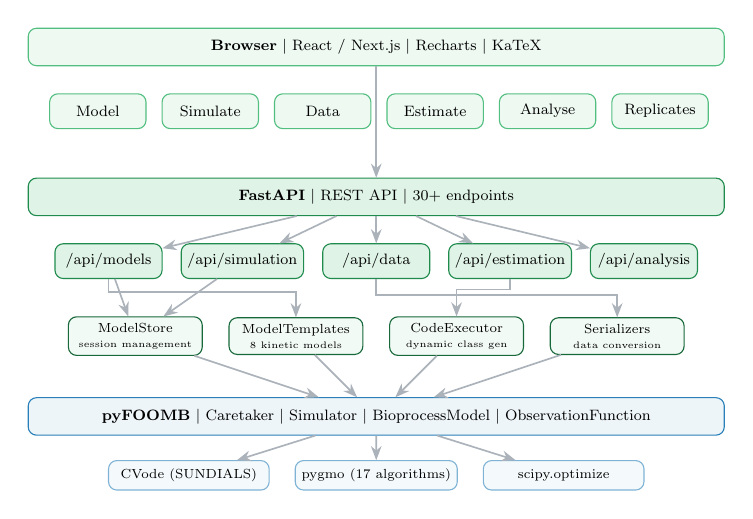
\begin{tikzpicture}[scale=0.68, every node/.style={scale=0.68, align=center},
    fe/.style={rectangle, rounded corners=3pt, minimum height=0.65cm,
      draw=donegreen!80, fill=donegreen!8, font=\footnotesize},
    be/.style={rectangle, rounded corners=3pt, minimum height=0.65cm,
      draw=donegreen!80!black, fill=donegreen!15, font=\footnotesize},
    svc/.style={rectangle, rounded corners=3pt, minimum height=0.65cm,
      draw=donegreen!60!black, fill=donegreen!6, font=\scriptsize},
    pf/.style={rectangle, rounded corners=3pt, minimum height=0.65cm,
      draw=accentblue, fill=accentblue!8, font=\footnotesize},
    sol/.style={rectangle, rounded corners=3pt, minimum height=0.55cm,
      draw=accentblue!60, fill=accentblue!5, font=\scriptsize},
    lbl/.style={font=\scriptsize\itshape, color=darkcharcoal!50},
    arr/.style={-{Stealth[length=1.8mm]}, color=darkcharcoal!40, semithick}
  ]
    % ── Browser
    \node[fe, minimum width=13cm, minimum height=0.7cm] (browser) at (0,0)
      {\textbf{Browser} $\vert$ React / Next.js $\vert$ Recharts $\vert$ KaTeX};

    % ── Frontend pages (evenly spaced)
    \node[fe, minimum width=1.8cm] (p1) at (-5.2,-1.2) {Model};
    \node[fe, minimum width=1.8cm] (p2) at (-3.1,-1.2) {Simulate};
    \node[fe, minimum width=1.8cm] (p3) at (-1,-1.2) {Data};
    \node[fe, minimum width=1.8cm] (p4) at (1.1,-1.2) {Estimate};
    \node[fe, minimum width=1.8cm] (p5) at (3.2,-1.2) {Analyse};
    \node[fe, minimum width=1.8cm] (p6) at (5.3,-1.2) {Replicates};

    % ── FastAPI
    \node[be, minimum width=13cm, minimum height=0.7cm] (api) at (0,-2.8)
      {\textbf{FastAPI} $\vert$ REST API $\vert$ 30+ endpoints};

    % ── Routers (evenly spaced)
    \node[be, minimum width=2cm] (r1) at (-5,-4) {/api/models};
    \node[be, minimum width=2cm] (r2) at (-2.5,-4) {/api/simulation};
    \node[be, minimum width=2cm] (r3) at (0,-4) {/api/data};
    \node[be, minimum width=2cm] (r4) at (2.5,-4) {/api/estimation};
    \node[be, minimum width=2cm] (r5) at (5,-4) {/api/analysis};

    % ── Services (4 services, evenly spaced)
    \node[svc, minimum width=2.5cm] (s1) at (-4.5,-5.4) {ModelStore\\{\tiny session management}};
    \node[svc, minimum width=2.5cm] (s2) at (-1.5,-5.4) {ModelTemplates\\{\tiny 8 kinetic models}};
    \node[svc, minimum width=2.5cm] (s3) at (1.5,-5.4) {CodeExecutor\\{\tiny dynamic class gen}};
    \node[svc, minimum width=2.5cm] (s4) at (4.5,-5.4) {Serializers\\{\tiny data conversion}};

    % ── pyFOOMB core
    \node[pf, minimum width=13cm, minimum height=0.7cm] (pfcore) at (0,-6.9)
      {\textbf{pyFOOMB} $\vert$ Caretaker $\vert$ Simulator $\vert$ BioprocessModel $\vert$ ObservationFunction};

    % ── Solvers
    \node[sol, minimum width=3cm] (cv) at (-3.5,-8) {CVode (SUNDIALS)};
    \node[sol, minimum width=3cm] (pg) at (0,-8) {pygmo (17 algorithms)};
    \node[sol, minimum width=3cm] (sp) at (3.5,-8) {scipy.optimize};

    % ── Arrows (clean vertical flow)
    \draw[arr] (browser) -- (api);
    \draw[arr] (api) -- (r1);
    \draw[arr] (api) -- (r2);
    \draw[arr] (api) -- (r3);
    \draw[arr] (api) -- (r4);
    \draw[arr] (api) -- (r5);
    \draw[arr] (r1) -- (s1);
    \draw[arr] (r1.south) -- ++(0,-0.25) -| (s2.north);
    \draw[arr] (r2) -- (s1);
    \draw[arr] (r4.south) -- ++(0,-0.2) -| (s3.north);
    \draw[arr] (r3.south) -- ++(0,-0.3) -| (s4.north);
    \draw[arr] (s1) -- (pfcore);
    \draw[arr] (s2) -- (pfcore);
    \draw[arr] (s3) -- (pfcore);
    \draw[arr] (s4) -- (pfcore);
    \draw[arr] (pfcore) -- (cv);
    \draw[arr] (pfcore) -- (pg);
    \draw[arr] (pfcore) -- (sp);
  \end{tikzpicture}
  \end{center}
\end{frame}

% ── Slide 7: GUI Workflow ─────────────────────────────────
\begin{frame}{GUI: Modelling Workflow}
  {\small The GUI provides a step-by-step pipeline from model definition to analysis:}

  \vspace{0.3cm}
  \begin{center}
  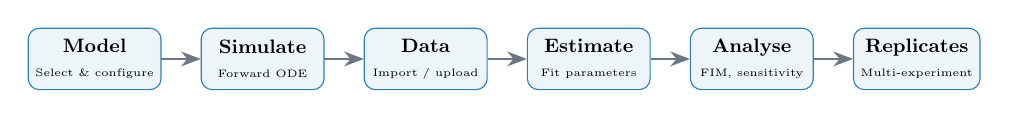
\begin{tikzpicture}[node distance=0.5cm, scale=0.78, every node/.style={scale=0.78, align=center},
    wfstep/.style={rectangle, rounded corners=4pt, minimum width=2cm, minimum height=1cm,
      draw=accentblue, fill=accentblue!8, font=\small}
  ]
    \node[wfstep] (m) {\textbf{Model}\\{\tiny Select \& configure}};
    \node[wfstep, right=of m] (s) {\textbf{Simulate}\\{\tiny Forward ODE}};
    \node[wfstep, right=of s] (d) {\textbf{Data}\\{\tiny Import / upload}};
    \node[wfstep, right=of d] (e) {\textbf{Estimate}\\{\tiny Fit parameters}};
    \node[wfstep, right=of e] (a) {\textbf{Analyse}\\{\tiny FIM, sensitivity}};
    \node[wfstep, right=of a] (r) {\textbf{Replicates}\\{\tiny Multi-experiment}};

    \draw[arrow] (m) -- (s);
    \draw[arrow] (s) -- (d);
    \draw[arrow] (d) -- (e);
    \draw[arrow] (e) -- (a);
    \draw[arrow] (a) -- (r);
  \end{tikzpicture}
  \end{center}

  \vspace{0.2cm}
  \begin{columns}[T]
    \begin{column}{0.48\textwidth}
      \textbf{Model Templates (8):}
      {\small
      \begin{itemize}
        \item Monod, Logistic, Exponential Growth
        \item Substrate Inhibition (Andrews)
        \item Contois, Double Monod
        \item Exponential Decay
        \item Fed-Batch Monod (with events)
      \end{itemize}
      }
    \end{column}
    \begin{column}{0.48\textwidth}
      \textbf{Estimation Methods (5):}
      {\small
      \begin{itemize}
        \item Local (scipy L-BFGS-B, Nelder-Mead)
        \item Global parallel (pygmo, 17 algorithms)
        \item Repeated local from random starts
        \item Monte Carlo sampling
        \item Parallelised Monte Carlo
      \end{itemize}
      }
    \end{column}
  \end{columns}
\end{frame}

% ── Slide 8: GUI Screenshot ───────────────────────────────
\begin{frame}{GUI: Interface}
  \begin{center}
    % Replace with your screenshot:
    % \includegraphics[width=0.85\textwidth]{gui_screenshot.png}
    {\large\textcolor{pendinggray}{[Place your GUI screenshot here]}}\\[0.3cm]
    {\small\textcolor{pendinggray}{Save as \texttt{gui\_screenshot.png} and uncomment the line above.}}
  \end{center}
\end{frame}


% ── Slide 9: μ–qp Relationship Models ─────────────────────
\begin{frame}{$\mu$--$q_p$ Relationship Models}
  The $\mu$--$q_p$ relationship governs how fast a cell produces product at a given growth rate.
  It determines the \textbf{optimal feeding strategy} in fed-batch.

  \vspace{0.2cm}
  \begin{columns}[T]
    \begin{column}{0.31\textwidth}
      \begin{block}{Linear}
        \begin{center}
          $q_p = \alpha \mu + \beta$
        \end{center}
        \vspace{0.1cm}
        {\small Growth-associated.\\Feed to maximise $\mu$.}
      \end{block}
    \end{column}
    \begin{column}{0.34\textwidth}
      \begin{block}{Bell-Shaped}
        \begin{center}
          $q_p = q_p^{max} e^{-\frac{(\mu - \mu_{opt})^2}{2\sigma^2}}$
        \end{center}
        \vspace{0.1cm}
        {\small Peak at $\mu_{opt}$.\\Maintain $\mu = \mu_{opt}$.}
      \end{block}
    \end{column}
    \begin{column}{0.31\textwidth}
      \begin{block}{Hyperbolic}
        \begin{center}
          $q_p = \frac{q_p^{max} \mu}{K_q + \mu}$
        \end{center}
        \vspace{0.1cm}
        {\small Saturates at high $\mu$.\\Flexible feeding.}
      \end{block}
    \end{column}
  \end{columns}

  \vspace{0.3cm}
  {\small We surveyed 9 products from literature across \textit{S.\ cerevisiae} and \textit{P.\ pastoris},
  and fitted each to one of these three models using \texttt{scipy.optimize.curve\_fit}.}
\end{frame}

% ── Slide 10: Literature Survey ───────────────────────────
\begin{frame}{Literature Survey: 9 Products, 2 Organisms}
  \vspace{-0.1cm}
  {\small $\mu$--$q_p$ data extracted from chemostat (CSTR) steady-state experiments at various dilution rates.}

  \vspace{0.2cm}
  \begin{center}
  \renewcommand{\arraystretch}{1.15}
  {\footnotesize
  \begin{tabular}{llllc}
    \toprule
    \textbf{Product} & \textbf{Organism} & \textbf{Model} & \textbf{Reference} & \textbf{$n$} \\
    \midrule
    Resveratrol              & \textit{S.\ cerevisiae} & Linear     & Vos et al.\ (2015)              & 5 \\
    VHH Antibody Fragments   & \textit{S.\ cerevisiae} & Linear     & Frenken et al.\ (1998)          & 6 \\
    Crl1 Lipase (Single-Copy) & \textit{P.\ pastoris}  & Linear     & Garrig\'{o}s-Mart.\ (2019)      & 7 \\
    \midrule
    EPG Polygalacturonase    & \textit{S.\ cerevisiae} & Bell       & Glauche et al.\ (2017)          & 10 \\
    Fab Antibody Fragment    & \textit{P.\ pastoris}   & Bell       & Rebnegger et al.\ (2014)        & 9 \\
    ROL Lipase               & \textit{P.\ pastoris}   & Bell       & Gasset et al.\ (2012)           & 8 \\
    \midrule
    Crl1 Lipase (Multi-Copy)  & \textit{P.\ pastoris}  & Hyperbolic & Garrig\'{o}s-Mart.\ (2019)      & 7 \\
    $\alpha$-Galactosidase    & \textit{S.\ cerevisiae} & Hyperbolic & Hensing et al.\ (1998)          & 8 \\
    GFP                      & \textit{P.\ pastoris}   & Hyperbolic & Mattanovich et al.\ (2021)      & 8 \\
    \bottomrule
  \end{tabular}
  }
  \end{center}

  \vspace{0.1cm}
  {\small $n$ = number of steady-state data points per product. Parameters fitted using \texttt{scipy.optimize.curve\_fit}.}
\end{frame}

% ── Slide 11: Extracted Data ──────────────────────────────
\begin{frame}{Extracted Data: $\mu$ and $q_p$ Ranges}
  \vspace{-0.1cm}
  {\small Data points digitised from each publication:}

  \vspace{0.2cm}
  \begin{center}
  \renewcommand{\arraystretch}{1.15}
  {\footnotesize
  \begin{tabular}{llcccc}
    \toprule
    \textbf{Product} & \textbf{Model} & \textbf{$\mu$ range (h$^{-1}$)} & \textbf{$q_p$ range} & \textbf{Unit} & \textbf{$R^2$} \\
    \midrule
    Resveratrol          & Linear & 0.025--0.15  & 0.003--0.024 & mmol/(g$\cdot$h) & 0.99 \\
    VHH Antibody         & Linear & 0.03--0.20   & 0.8--6.0     & mg/(g$\cdot$h)   & 0.99 \\
    Crl1 Lipase (SCC)    & Linear & 0.02--0.15   & 5.0--48.0    & AU/(g$\cdot$h)   & 0.99 \\
    \midrule
    EPG                  & Bell   & 0.01--0.35   & 50--400      & U/(g$\cdot$h)    & 0.84 \\
    Fab Fragment         & Bell   & 0.005--0.15  & 1.2--14.0    & mg/(g$\cdot$h)   & 0.96 \\
    ROL Lipase           & Bell   & 0.01--0.12   & 8.0--40.0    & AU/(g$\cdot$h)   & 0.92 \\
    \midrule
    Crl1 Lipase (MCC)    & Hyperbolic & 0.02--0.15   & 20--138      & AU/(g$\cdot$h)   & 0.99 \\
    $\alpha$-Galactosidase & Hyperbolic & 0.02--0.30   & 5.0--43.0    & U/(g$\cdot$h)    & 0.99 \\
    GFP                  & Hyperbolic & 0.01--0.18   & 5.0--60.0    & RFU/(g$\cdot$h)  & 0.99 \\
    \bottomrule
  \end{tabular}
  }
  \end{center}

  \vspace{0.15cm}
  {\small All data obtained from continuous cultures where dilution rate $D = \mu$ at steady state.
  Fitted parameters: $\alpha, \beta$ (linear); $q_p^{max}, \mu_{opt}, \sigma$ (bell); $q_p^{max}, K_q$ (hyperbolic).}
\end{frame}
% ── Slide 12: μ–qp Plot ──────────────────────────────────
\begin{frame}{$\mu$--$q_p$ Fitting Results}
  \vfill
  \begin{center}
    
\includegraphics[height=0.82\textheight]{mu_qp_relationships.png}
  \end{center}
  \vfill
\end{frame}

% ── Slide 12: XPS Simulation ─────────────────────────────
\begin{frame}{Batch X, S, P Profile Simulation}
  From the fitted $\mu$--$q_p$ parameters, we simulated full batch dynamics for each product.

  \vspace{0.2cm}
  \begin{columns}[T]
    \begin{column}{0.52\textwidth}
      \textbf{ODE System (Monod batch):}
      \begin{align*}
        \frac{dX}{dt} &= \mu \cdot X \\[3pt]
        \frac{dS}{dt} &= -\frac{\mu}{Y_{X/S}} \cdot X \\[3pt]
        \frac{dP}{dt} &= q_p(\mu) \cdot X
      \end{align*}
      where $\mu = \mu_{max} \cdot \dfrac{S}{K_S + S}$

      \vspace{0.15cm}
      {\small Integrated using \texttt{scipy.integrate.solve\_ivp} (RK45).}
    \end{column}
    \begin{column}{0.44\textwidth}
      \textbf{Organism-Specific Parameters:}

      \vspace{0.15cm}
      {\small
      \begin{tabular}{lcc}
        \toprule
        & \textit{S.c.} & \textit{P.p.} \\
        \midrule
        $\mu_{max}$ (h$^{-1}$) & 0.40 & 0.20 \\
        $K_S$ (g/L) & 0.10 & 0.05 \\
        $Y_{X/S}$ (g/g) & 0.50 & 0.45 \\
        \bottomrule
      \end{tabular}
      }

      \vspace{0.15cm}
      {\small $X_0 = 0.1$ g/L, $S_0 = 20$ g/L, $P_0 = 0$}
    \end{column}
  \end{columns}
\end{frame}

% ── Slide 13: XPS Plot ───────────────────────────────────
\begin{frame}{XPS Simulation Results}
  \vfill
  \begin{center}
    
\includegraphics[height=0.82\textheight]{xps_validated_profiles.png}
  \end{center}
  \vfill
\end{frame}

% ── Slide 14: Future Roadmap ─────────────────────────────
\begin{frame}{Project Roadmap}
  \vspace{-0.1cm}
  \begin{center}
  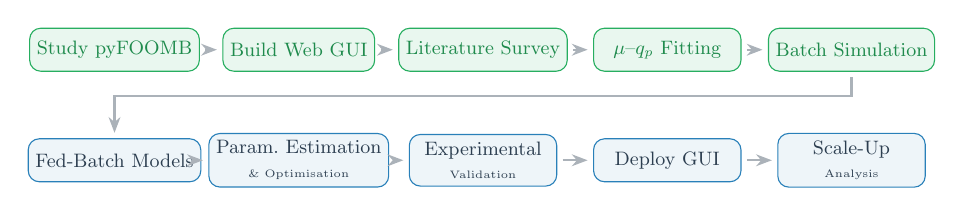
\begin{tikzpicture}[
    scale=0.78, every node/.style={scale=0.78, align=center},
    doneblock/.style={rectangle, rounded corners=4pt, minimum width=2.4cm, minimum height=0.7cm,
      draw=donegreen, fill=donegreen!10, font=\small, text=donegreen!80!black},
    pendblock/.style={rectangle, rounded corners=4pt, minimum width=2.4cm, minimum height=0.7cm,
      draw=accentblue, fill=accentblue!8, font=\small, text=darkcharcoal},
    arr/.style={-{Stealth[length=2mm]}, thick, color=darkcharcoal!40, shorten >=2pt, shorten <=2pt}
  ]
    % Row 1: Completed (equal 3cm spacing)
    \node[doneblock] (a1) at (0,0) {Study pyFOOMB};
    \node[doneblock] (a2) at (3,0) {Build Web GUI};
    \node[doneblock] (a3) at (6,0) {Literature Survey};
    \node[doneblock] (a4) at (9,0) {$\mu$--$q_p$ Fitting};
    \node[doneblock] (a5) at (12,0) {Batch Simulation};

    \draw[arr] (a1) -- (a2);
    \draw[arr] (a2) -- (a3);
    \draw[arr] (a3) -- (a4);
    \draw[arr] (a4) -- (a5);

    % Row 2: Next (equal 3cm spacing, same x positions)
    \node[pendblock] (b1) at (0,-1.8) {Fed-Batch Models};
    \node[pendblock] (b2) at (3,-1.8) {Param.\ Estimation\\{\tiny \& Optimisation}};
    \node[pendblock] (b3) at (6,-1.8) {Experimental\\{\tiny Validation}};
    \node[pendblock] (b4) at (9,-1.8) {Deploy GUI};
    \node[pendblock] (b5) at (12,-1.8) {Scale-Up\\{\tiny Analysis}};

    % Right-angle connector from row 1 end to row 2 start
    \draw[arr] (a5.south) -- ++(0,-0.4) -| (b1.north);

    \draw[arr] (b1) -- (b2);
    \draw[arr] (b2) -- (b3);
    \draw[arr] (b3) -- (b4);
    \draw[arr] (b4) -- (b5);
  \end{tikzpicture}
  \end{center}

  \vspace{0.2cm}
  \begin{columns}[T]
    \begin{column}{0.48\textwidth}
      \textbf{Completed this semester:}
      {\small
      \begin{itemize}
        \item[\textcolor{donegreen}{\checkmark}] Full pyFOOMB web GUI
        \item[\textcolor{donegreen}{\checkmark}] 9-product $\mu$--$q_p$ literature survey
        \item[\textcolor{donegreen}{\checkmark}] Batch XPS profile simulations
      \end{itemize}
      }
    \end{column}
    \begin{column}{0.48\textwidth}
      \textbf{Planned next:}
      {\small
      \begin{itemize}
        \item[\textcolor{accentblue}{$\circ$}] Fed-batch ODE models with feed events
        \item[\textcolor{accentblue}{$\circ$}] Fit \& optimise feed profiles
        \item[\textcolor{accentblue}{$\circ$}] Validate against experimental data
        \item[\textcolor{accentblue}{$\circ$}] Deploy GUI
      \end{itemize}
      }
    \end{column}
  \end{columns}
\end{frame}

% ── Slide 15: Thank You ──────────────────────────────────
\begin{frame}[plain]
  \vfill
  \begin{center}
    {\LARGE\bfseries\color{darkcharcoal} Thank You}\\[0.6cm]
    {\large\color{accentblue} Questions?}\\[1cm]
    \begin{tabular}{rl}
      \textbf{Student:} & Yashashwi Singhania (23014019) \\
      \textbf{Guide:} & Dr.\ Sharon Mano Pappu J. \\
      \textbf{Lab:} & BPDD, Dept.\ of Biochemical Engineering \\
      \textbf{Institute:} & IIT (BHU) Varanasi \\
    \end{tabular}\\[0.8cm]
    {\small\color{darkcharcoal!60} April 2026}
  \end{center}
  \vfill
\end{frame}

\end{document}
